\begin{frame}{}
\begin{center}
    \Large
    \textbf{Integration of Low-Cost Sensor Data}
\end{center}
\end{frame}

\begin{frame}{Objectives}
    \begin{itemize}
        \item Are low-cost sensor data valuable in PM\tsub{2.5} modeling?
        \begin{itemize}
            \item Do they provide new information about pollution?
        \end{itemize}
        \item If so, how can they be used in the model?
        \begin{itemize}
            \item How to deal with their larger and unknown uncertainty?
        \end{itemize}
    \end{itemize}
\end{frame}

\begin{frame}{Modeling Strategy}
\begin{minipage}{0.5\textwidth}
    \footnotesize
    \begin{itemize}
        \item Modeling period: 2018
        \item Modeling domain: California at a 1$\times$1 km$^2$ grid
        \item 157 \textbf{AQS} stations with 51K daily and 0.5M hourly records (gold-standard)
        \item 2,090 \textbf{PurpleAir} sensors with 5.8M hourly records (lower data quality)
        \item 26 ``collocated'' AQS/PurpleAir sites with $>$ 100K paired hourly records
    \end{itemize}
\end{minipage}
\begin{minipage}{0.48\textwidth}
    \includegraphics[width=\textwidth]{img/ca.jpg}
\end{minipage}
\end{frame}

\begin{frame}{First Step: Calibration}
    Calibration: Minimizing the overall disagreement between AQS and PurpleAir
    \begin{itemize}
        \item Match AQS and PurpleAir sites within a distance of 500 m
        \item Build Geographically Weighted Regression (GWR) with \textbf{temperature}, \textbf{humidity}, and \textbf{total operational time} as covariates to locally calibrate the sensors
    \end{itemize}
    \begin{block}{Calibration Equation}
    \small
    $AQS\,PM_{2.5} = \beta_0 + \beta_1\cdot PurpleAir\,PM_{2.5} + \beta_2\cdot T + \beta_3\cdot RH + \beta_4\cdot Opl.\,Time$
    \end{block}
\end{frame}

\begin{frame}{Effect of calibration}
    \begin{itemize}
        \item Reduced the overall bias to $\sim 0 \mu g/m^3$
        \item Reduced the residual variance by $\sim$40\%
        \item Depicted quantitative relationships between the bias and the covariates
    \end{itemize}
    \begin{center}
        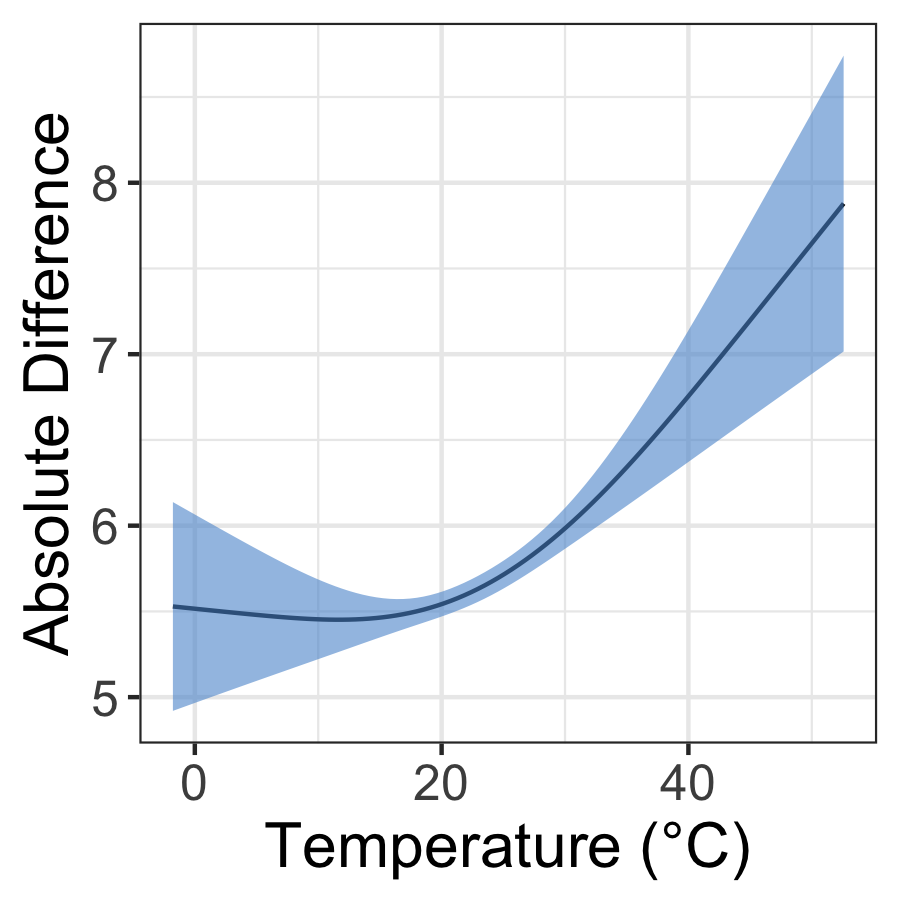
\includegraphics[width=0.32\textwidth]{img/temp.png}
        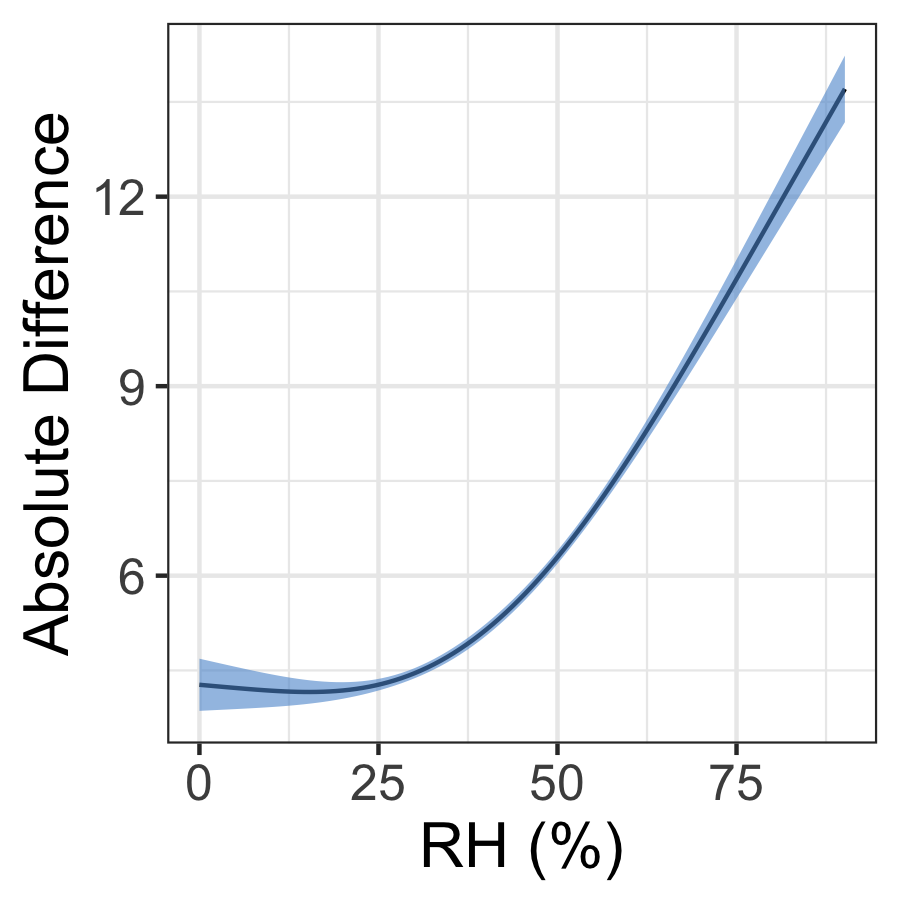
\includegraphics[width=0.32\textwidth]{img/rh.png}
        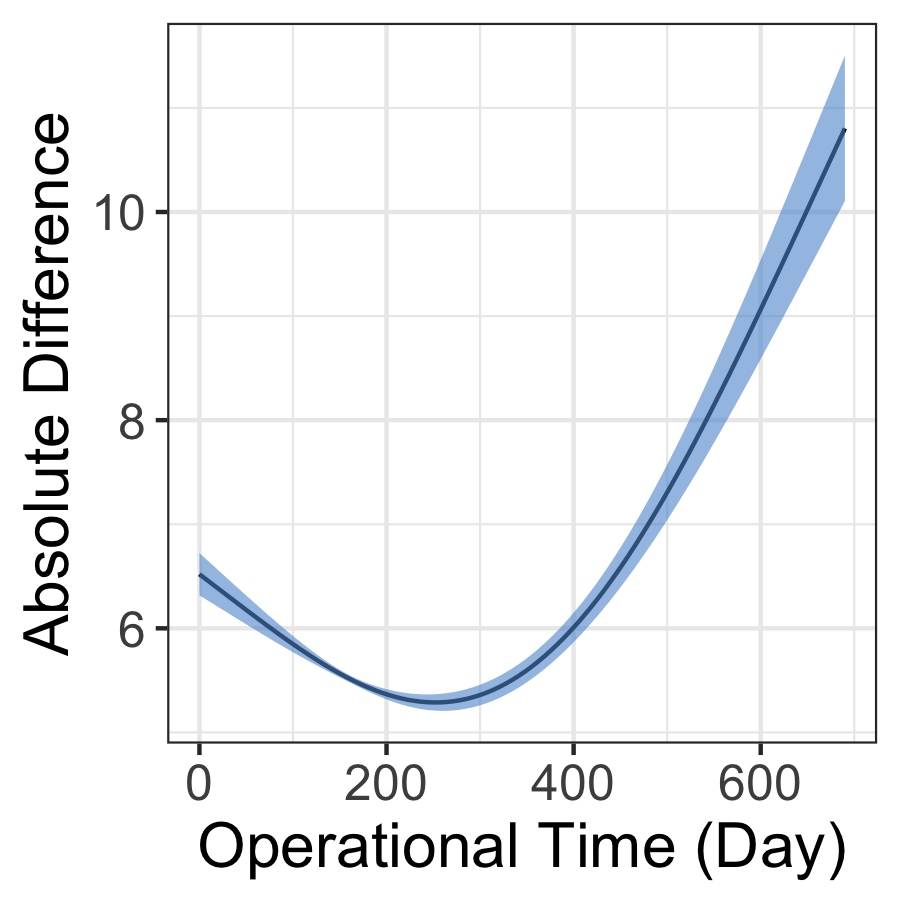
\includegraphics[width=0.32\textwidth]{img/time.png}
    \end{center}
\end{frame}

\begin{frame}{Second Step: Weighted Modeling}
    \begin{itemize}
        \item A weighted random forest model (1-km, daily)
        \item Daily Ground-level PM\tsub{2.5} (Dependent Variable)
        \begin{itemize}
            \item AQS: $w=1$
            \item PurpleAir: $\mathbf{w \approx 0.2}$
        \end{itemize}
    \end{itemize}
    \gatherblock{w=\rho\cdot\frac{\sigma^2}{\sigma^2+\tau_i^2}}
    \begin{center}
        $\rho$ - the \textbf{data-driven} scale factor
    \end{center}
    \begin{block}{Model Structure}
    \footnotesize
    $Ground\, PM_{2.5} = f(AOD, Meteorological, Land\operatorname{-}Cover, Population, Traffic, ...)$
    \end{block}
\end{frame}

\begin{frame}{Model predictions}
\begin{minipage}{0.44\textwidth}
    \begin{minipage}{\textwidth}
        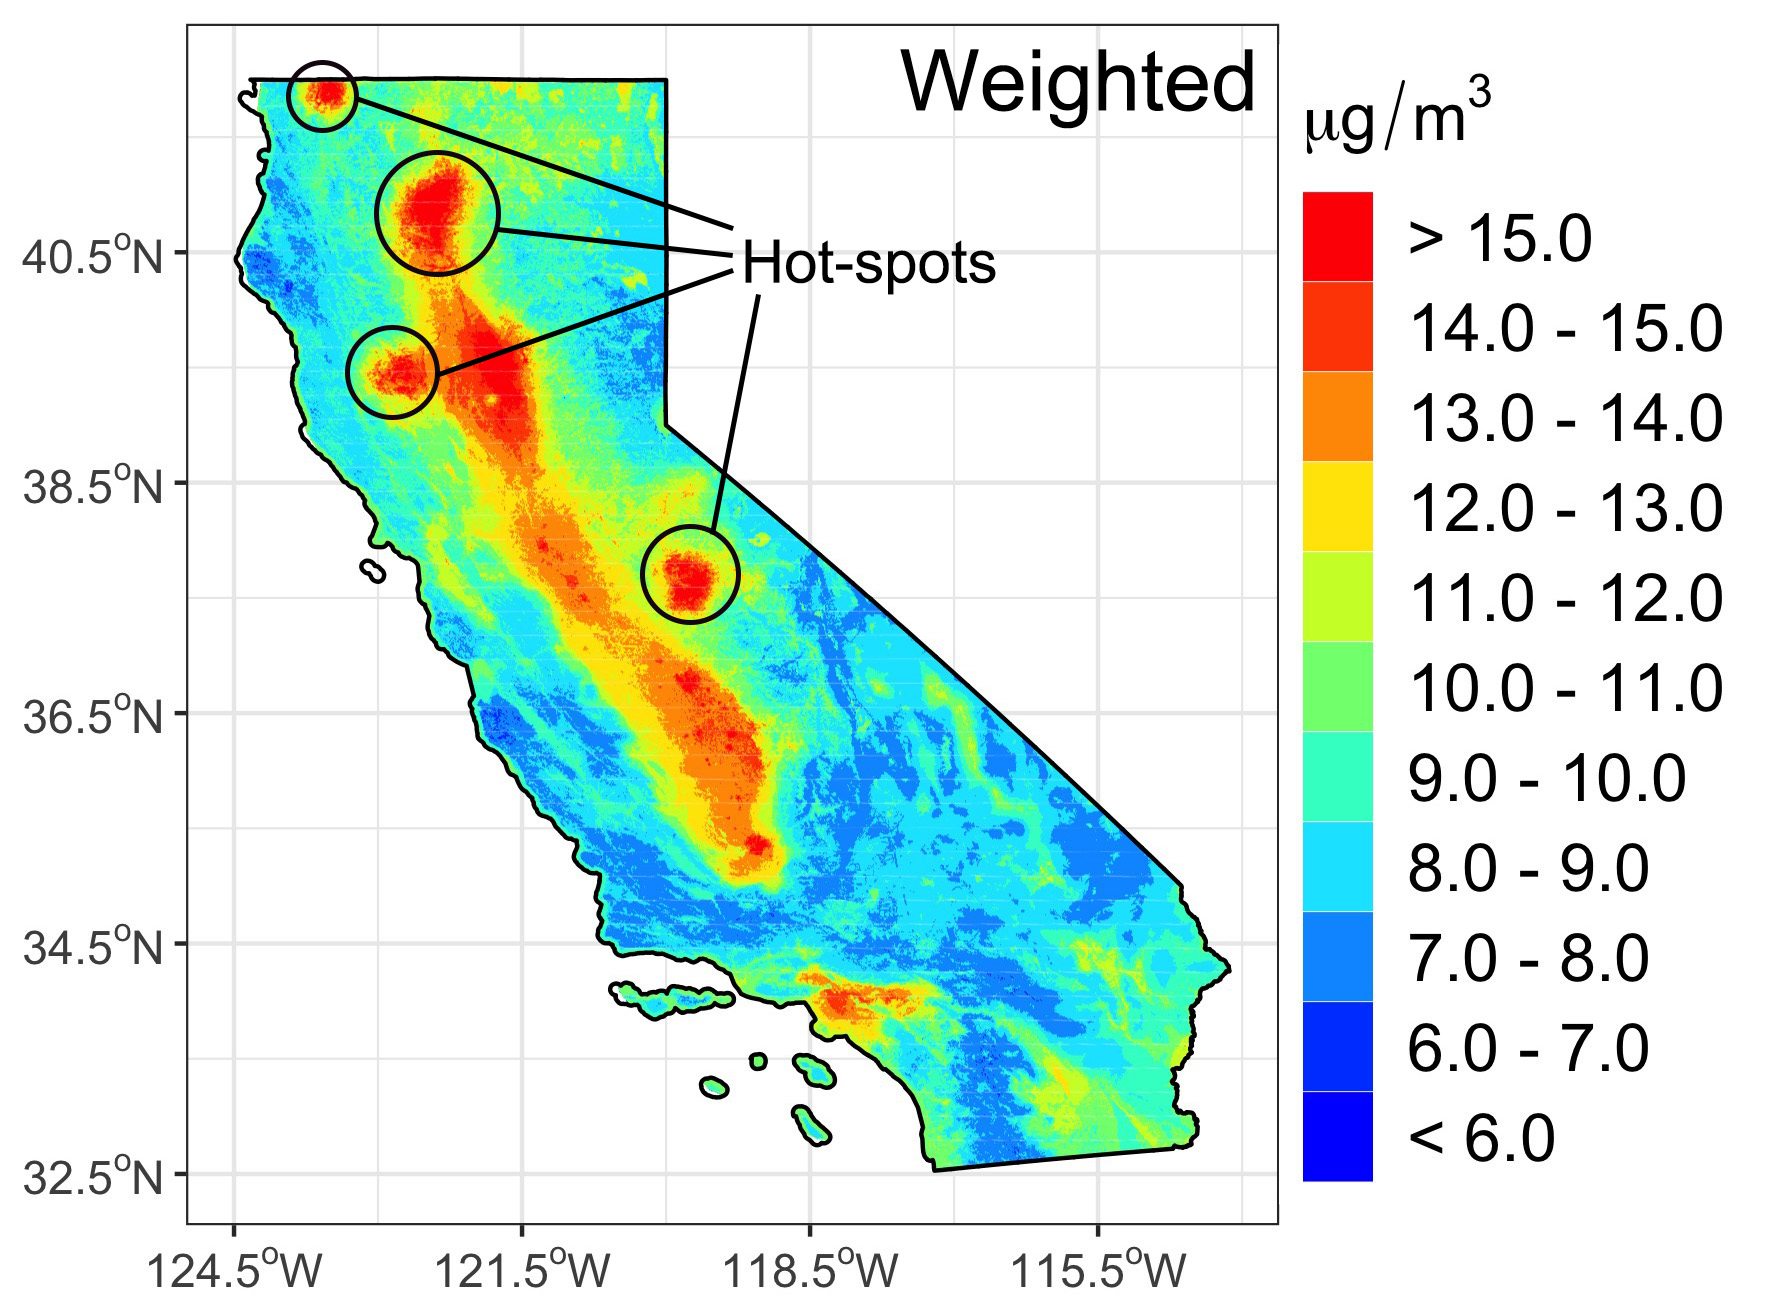
\includegraphics[width=\textwidth]{img/w.jpg}
    \end{minipage}
    \begin{minipage}{\textwidth}
        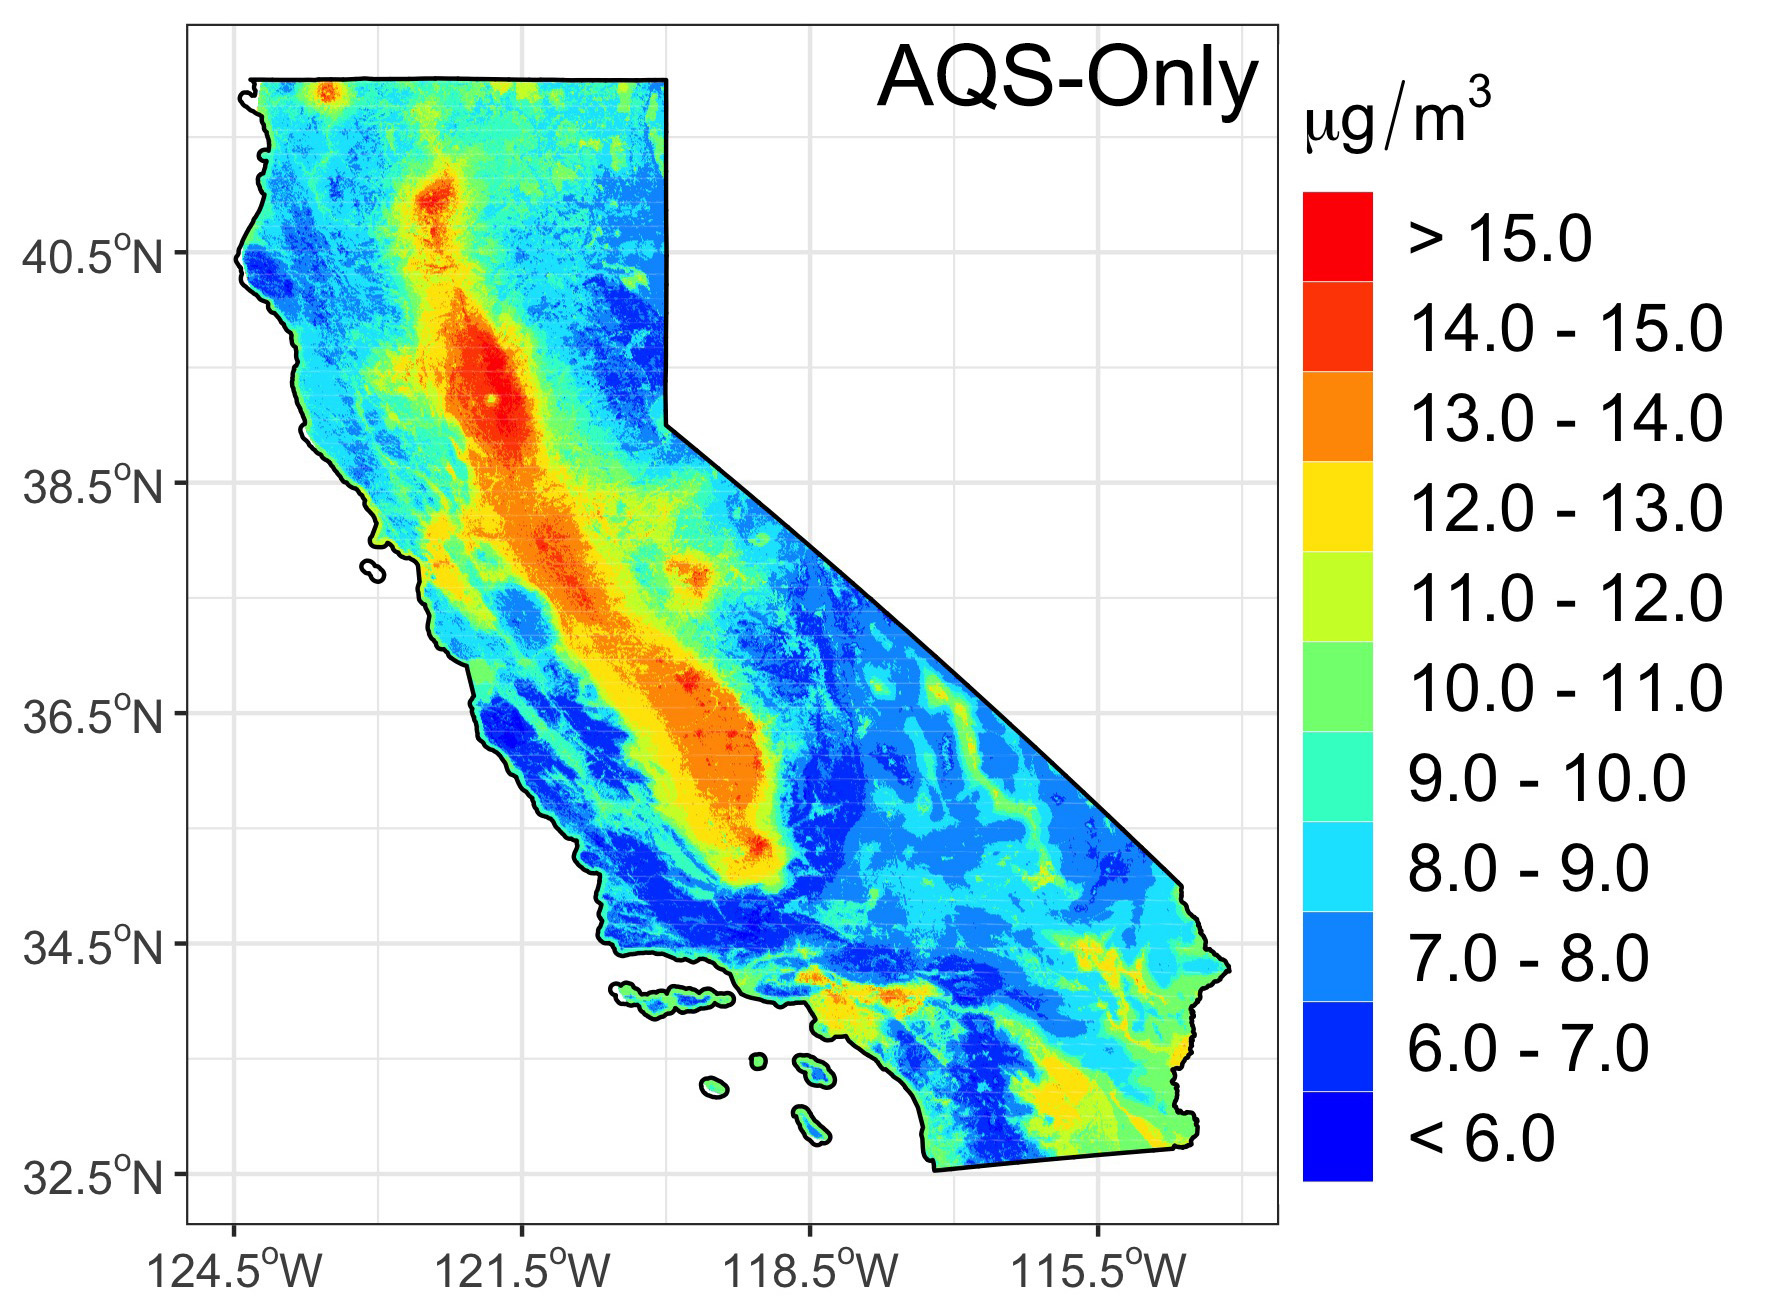
\includegraphics[width=\textwidth]{img/aqs.jpg}
    \end{minipage}
\end{minipage}
\begin{minipage}{0.54\textwidth}
    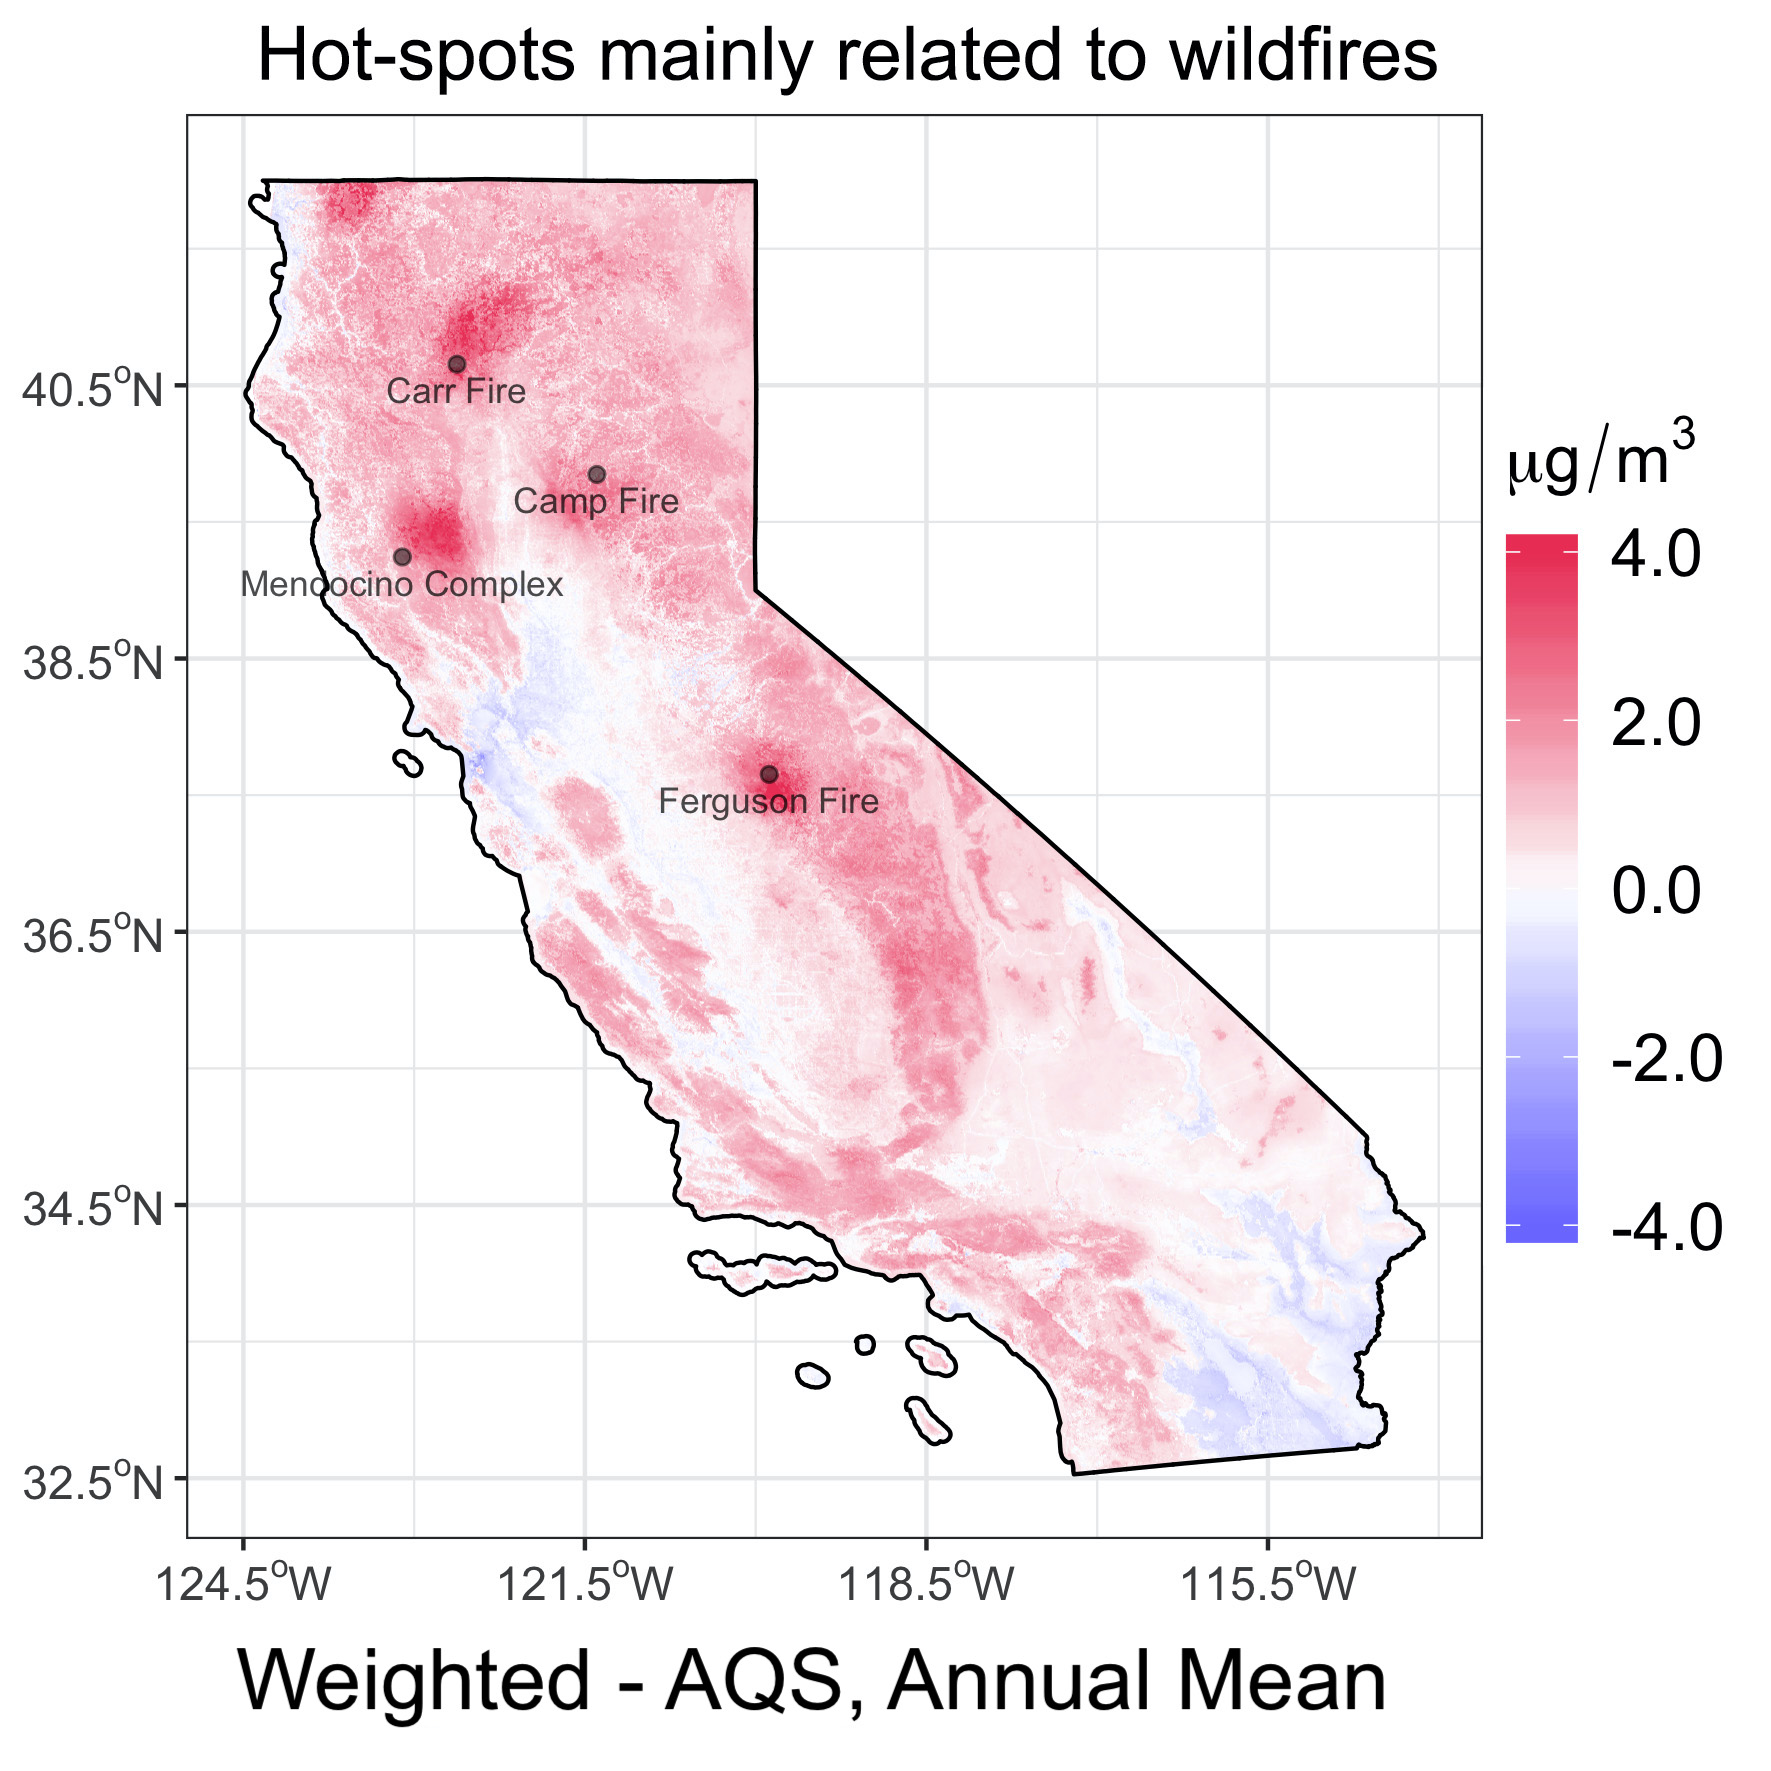
\includegraphics[width=\textwidth]{img/aqs_w.jpg}
\end{minipage}
\end{frame}

\begin{frame}{Summary}
    \begin{itemize}
        \item The negative impact of residual errors in low-cost sensor data can be mitigated by weighting to allow the integration of heterogeneous ground data in PM\tsub{2.5} modeling.
        \item The proposed two-step integration framework can be generalized to other regions with limited regulatory stations to improve exposure assessment.
        \item This framework can also be informative to other citizen-science applications to combine few gold-standard data and a large amount of volunteer-generated data.
    \end{itemize}
    \vspace{0.2cm}
    \begin{spacing}{0.3}
    \scriptsize
    \textbf{Bi, J.}, Wildani, A., Chang, H.H., \& Liu, Y. Incorporating Low-Cost Sensor Measurements into High-Resolution PM\tsub{2.5} Modeling at a Large Spatial Scale. \textit{Environmental Science \& Technology}, 10.1021/acs.est.9b06046.
    
    \vspace{0.2cm}
    
    \textbf{Bi, J.}, Stowell, J., Seto, E. Y. W., English, P. B., Al-Hamdan, M. Z., Kinney, P. L., Freedman, F. R., \& Liu, Y. (2020). Contribution of Low-Cost Sensor Measurements to the Prediction of PM\tsub{2.5} Levels: A Case Study in Imperial County, California, USA. \textit{Environmental Research}, 180, 108810.

    \end{spacing}
\end{frame}